\section{Введение}
В лабораторной работе требуется выбрать один из предложенных наборов данных для бинарной классификации, выполнить предварительную обработку, построить графики описательной статистики и разделить наблюдения на обучающую и тестовую выборки. Логистическую регрессию необходимо реализовать без готовых алгоритмов машинного обучения: вычислять сигмоиду и логарифмическую функцию потерь, обучать модель градиентным спуском и изменять шаг и число итераций. Дополнительно исследуется метод оптимизации. Каждая конфигурация оценивается по Accuracy, Precision, Recall и F1, после чего анализируется влияние гиперпараметров.

Цель работы --- выполнить эти этапы на наборе Pima Indians Diabetes и сравнить градиентный спуск с методом Ньютона. Целевой признак \code{Outcome} принимает значения 0 и 1; положительным считается класс 1.

Реализованы устойчивое вычисление сигмоиды и log loss, полный градиентный спуск, метод Ньютона, предобработка и четыре метрики. Рассмотрена 21 комбинация гиперпараметров. Выбранная по validation log loss модель GD с $\alpha=0.1$, $T=100$ после переобучения на train дала на test Accuracy $0.7792$, Precision $0.7381$, Recall $0.5741$ и F1 $0.6458$.

\section{Описание метода}
\subsection{Линейная и логистическая регрессия}

Обе модели строят линейный предиктор $z_i=\widetilde{x}_i^\mathsf{T}w$, где первый элемент $\widetilde{x}_i$ равен 1. В линейной регрессии он непосредственно задаёт прогноз количественного отклика. В логистической регрессии он определяет логарифм шансов бинарного события:
\[
 \log\frac{p_i}{1-p_i}=\widetilde{x}_i^\mathsf{T}w,
 \qquad p_i=P(y_i=1\mid x_i).
\]
Для оценки коэффициентов линейной регрессии часто используют формулу МНК $(X^\mathsf{T}X)^{-1}X^\mathsf{T}y$. В логистической модели параметры находятся численной минимизацией отрицательного логарифма правдоподобия Бернулли. Нормальность и постоянная дисперсия ошибок линейной регрессии не распространяются на бинарный отклик, для которого $\operatorname{Var}(y_i\mid x_i)=p_i(1-p_i)$.

\subsection{Гипотеза, потери и решение}
Вероятность вычисляется сигмоидой:
\[
 \sigma(z)=\frac1{1+e^{-z}}
 =\begin{cases}(1+e^{-z})^{-1},&z\geq0,\\e^z/(1+e^z),&z<0.\end{cases}
\]
Разделение ветвей исключает переполнение экспоненты для больших по модулю логитов. Решение принимается при фиксированном пороге $0.5$: $\widehat y_i=\mathbf1[p_i\geq0.5]$.
\begin{align*}
 L(w)&=-\frac1n\sum_{i=1}^n\big[y_i\log p_i+(1-y_i)\log(1-p_i)\big]\\
 &=\frac1n\sum_{i=1}^n\big[\log(1+e^{z_i})-y_i z_i\big].
\end{align*}
В коде $\log(1+e^z)$ вычисляется через \code{np.logaddexp(0, z)}, поэтому не требуется искусственно обрезать вероятности перед логарифмированием. Регуляризация в целевую функцию не добавлена.

\subsection{Методы оптимизации}
Для матрицы $X$, включающей столбец единиц, градиент и гессиан имеют вид
\[
 g=\frac1nX^\mathsf{T}(p-y),\qquad
 H=\frac1nX^\mathsf{T}DX,\quad D_{ii}=p_i(1-p_i).
\]
Полный градиентный спуск обновляет все параметры по всей обучающей выборке:
\[
 w^{(t+1)}=w^{(t)}-\alpha g^{(t)}.
\]
Метод Ньютона учитывает кривизну функции потерь:
\[
 (H^{(t)}+10^{-8}I)d^{(t)}=g^{(t)},\qquad
 w^{(t+1)}=w^{(t)}-\alpha d^{(t)}.
\]
Система решается \code{np.linalg.solve}; обратная матрица явно не строится. Добавка $10^{-8}I$ стабилизирует линейную систему и не является штрафом в $L(w)$. Для Ньютона $\alpha$ --- множитель шага: $\alpha=1$ соответствует полному шагу, меньшие значения --- демпфированию. Обе реализации начинают с $w=0$ и выполняют ровно $T$ итераций. Автоматической ранней остановки и поиска длины шага нет.

При $d$ признаках одна итерация GD требует порядка $O(nd)$ операций, а Ньютона --- $O(nd^2+d^3)$. Для восьми признаков решение системы $9\times9$ невелико; при большом $d$ преимущество по числу итераций не означает преимущество по времени. В работе сравнивается сходимость по итерациям, аппаратный бенчмарк не проводился.

\subsection{Метрики}
Строки матрицы ошибок соответствуют истинным классам, столбцы --- предсказанным; порядок классов $0,1$:
\[
 C=\begin{pmatrix}TN&FP\\FN&TP\end{pmatrix}.
\]
\[
 \mathrm{Accuracy}=\frac{TP+TN}{n},\quad
 \mathrm{Precision}=\frac{TP}{TP+FP},\quad
 \mathrm{Recall}=\frac{TP}{TP+FN},\quad
 \mathrm{F1}=\frac{2TP}{2TP+FP+FN}.
\]
При нулевом знаменателе Precision, Recall или F1 возвращается 0. Все метрики и матрица ошибок реализованы вручную на NumPy. Accuracy учитывает оба класса; Recall показывает долю найденных положительных объектов, Precision --- долю верных положительных прогнозов. F1 объединяет Precision и Recall, но не использует число TN.

\section{Псевдокод метода}
\subsection{Обучение модели}
\begin{enumerate}
\item Получить $X$, $y$, метод, шаг $\alpha>0$, число итераций $T$; положить $w=0$.
\item Сохранить начальное значение $L(w)$.
\item Для $t=1,\ldots,T$:
\begin{enumerate}
\item Вычислить $z=Xw$, $p=\sigma(z)$, $g=X^\mathsf{T}(p-y)/n$.
\item Для GD положить $d=g$. Для Ньютона построить $H$ и решить $(H+10^{-8}I)d=g$.
\item Обновить $w\leftarrow w-\alpha d$, вычислить и сохранить $L(w)$.
\item Если потери не конечны, завершить обучение с сообщением об ошибке.
\end{enumerate}
\item Вернуть веса и историю потерь; прогнозировать класс по порогу $0.5$.
\end{enumerate}

\subsection{План эксперимента}
\begin{enumerate}
\item Загрузить CSV; проверить размер, целевые метки, пропуски и дубликаты; сохранить статистику.
\item Стратифицированно разделить данные на train/test с seed 42, затем train на fit/validation с seed 43.
\item На fit оценить медианы, средние и стандартные отклонения. Преобразовать fit и validation с этими параметрами.
\item Обучить каждую из 21 конфигураций на fit. Выбрать минимум validation log loss; при точном равенстве оставить первую конфигурацию в заданном порядке.
\item Зафиксировать выбор до оценки test. Заново оценить предобработку на полном train.
\item Для каждой конфигурации заново обучить модель на train и вычислить метрики на test, как требует задание. Не менять выбор по этим результатам.
\item Сохранить таблицы, индексы разбиения, веса, вероятности и графики.
\end{enumerate}

\section{Результаты выполнения}
\subsection{Данные и предварительная обработка}
Исходный набор содержит 768 наблюдений, восемь числовых признаков и целевой столбец. Все наблюдения относятся к женщинам происхождения Pima в возрасте не менее 21 года. Класс 0 представлен 500 объектами, класс 1 --- 268. В данных нет явных NaN и полных дубликатов строк.

\begin{table}[H]\centering\small
\begin{tabularx}{\linewidth}{lX}
\toprule Признак & Содержание\\\midrule
Pregnancies & Число беременностей.\\
Glucose & Концентрация глюкозы через 2 часа в тесте толерантности.\\
BloodPressure & Диастолическое давление, мм рт. ст.\\
SkinThickness & Толщина кожной складки трицепса, мм.\\
Insulin & Уровень инсулина через 2 часа, мкЕд/мл.\\
BMI & Индекс массы тела, кг/м$^2$.\\
DiabetesPedigreeFunction & Числовой показатель наследственности.\\
Age & Возраст, годы.\\\bottomrule
\end{tabularx}
\caption{Использованные признаки.}
\end{table}

Нули в Glucose, BloodPressure, SkinThickness, Insulin и BMI трактуются как отсутствующие измерения. Их количества: 5, 35, 227, 374 и 11 соответственно. Нулевая беременность является допустимым значением и сохраняется. Категориальных входных признаков нет, поэтому дополнительное кодирование не требуется.

Пропуски заполняются медианами обучения; после заполнения выполняется стандартизация $x'_j=(x_j-\mu_j)/s_j$. Для масштабирования используется $s_j$ с \code{ddof=0}; если $s_j=0$, масштаб заменяется на 1. Медианы и масштабы test не участвуют в обучении. Статистические графики описывают весь набор, но не используются для выбора признаков или параметров. Все восемь признаков заданы заранее; строки и выбросы не удаляются.

\begin{figure}[H]\centering
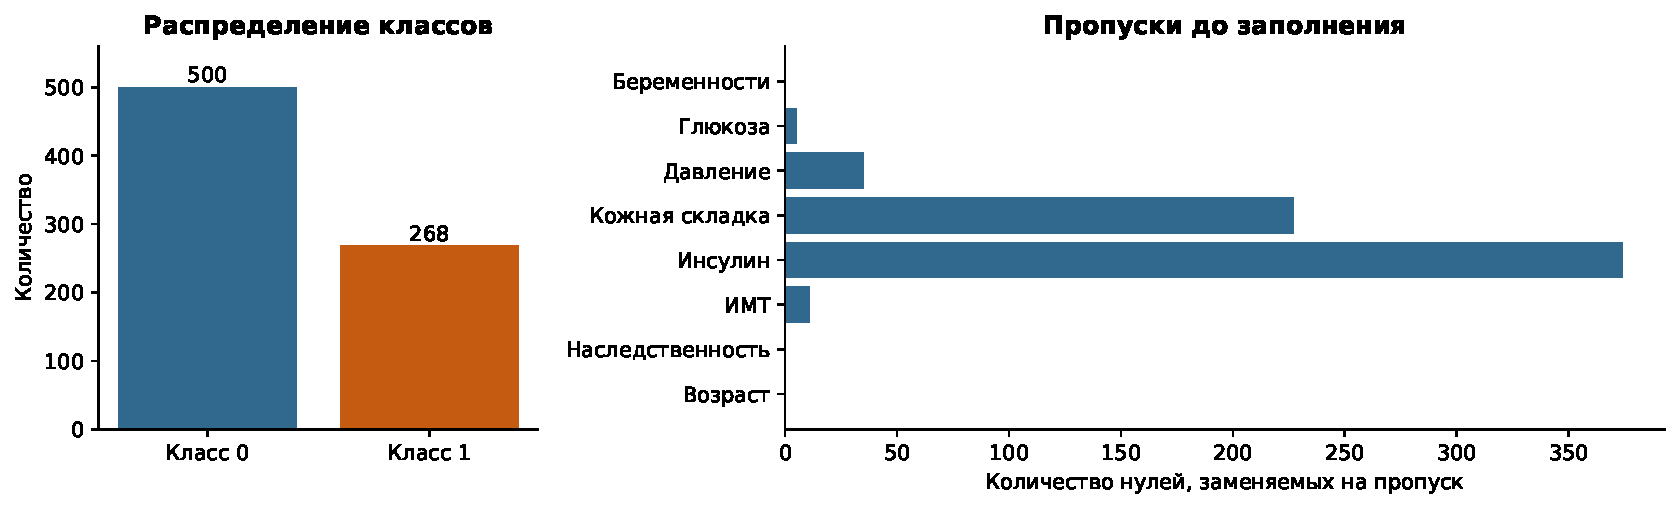
\includegraphics[width=\linewidth]{figures/missing_classes.pdf}
\caption{Баланс классов и отсутствующие измерения.}
\end{figure}

\subsection{Описательная статистика и визуализация}
В таблице приведены статистики по наблюдаемым значениям после обозначения отсутствующих измерений как NaN, до заполнения. $s$ --- выборочное стандартное отклонение (\code{ddof=1}); Q1, Q2 и Q3 --- квантили 0.25, 0.50 и 0.75.
\begin{table}[H]\centering\scriptsize
\begin{tabular}{lrrrrrrrr}
\toprule
Признак & n & Среднее & s & min & Q1 & Q2 & Q3 & max \\
\midrule
Беременности & 768 & 3.85 & 3.37 & 0.00 & 1.00 & 3.00 & 6.00 & 17.00 \\
Глюкоза & 763 & 121.69 & 30.54 & 44.00 & 99.00 & 117.00 & 141.00 & 199.00 \\
Давление & 733 & 72.41 & 12.38 & 24.00 & 64.00 & 72.00 & 80.00 & 122.00 \\
Кожная складка & 541 & 29.15 & 10.48 & 7.00 & 22.00 & 29.00 & 36.00 & 99.00 \\
Инсулин & 394 & 155.55 & 118.78 & 14.00 & 76.25 & 125.00 & 190.00 & 846.00 \\
ИМТ & 757 & 32.46 & 6.92 & 18.20 & 27.50 & 32.30 & 36.60 & 67.10 \\
Наследственность & 768 & 0.47 & 0.33 & 0.08 & 0.24 & 0.37 & 0.63 & 2.42 \\
Возраст & 768 & 33.24 & 11.76 & 21.00 & 24.00 & 29.00 & 41.00 & 81.00 \\
\bottomrule
\end{tabular}

\caption{Количество, среднее, стандартное отклонение, минимум, максимум и квантили.}
\end{table}
\begin{figure}[H]\centering
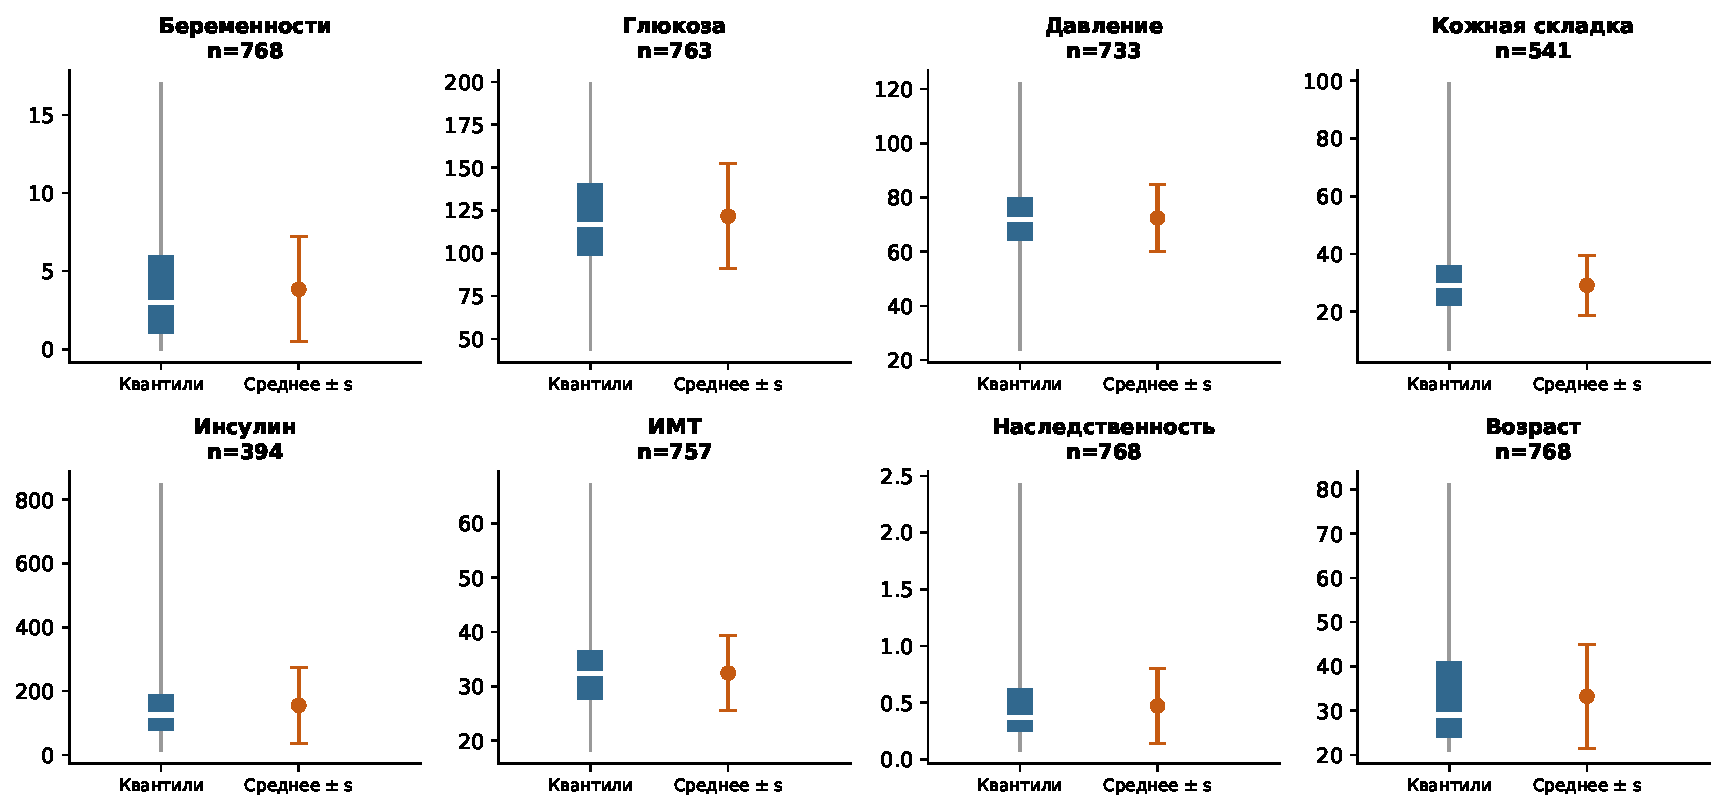
\includegraphics[width=\linewidth]{figures/statistics.pdf}
\caption{Все требуемые статистики: число наблюдений в заголовках; тонкий отрезок min--max; толстый Q1--Q3; белая отметка --- медиана; оранжевая точка и интервал --- среднее $\pm s$.}
\end{figure}
\begin{figure}[H]\centering
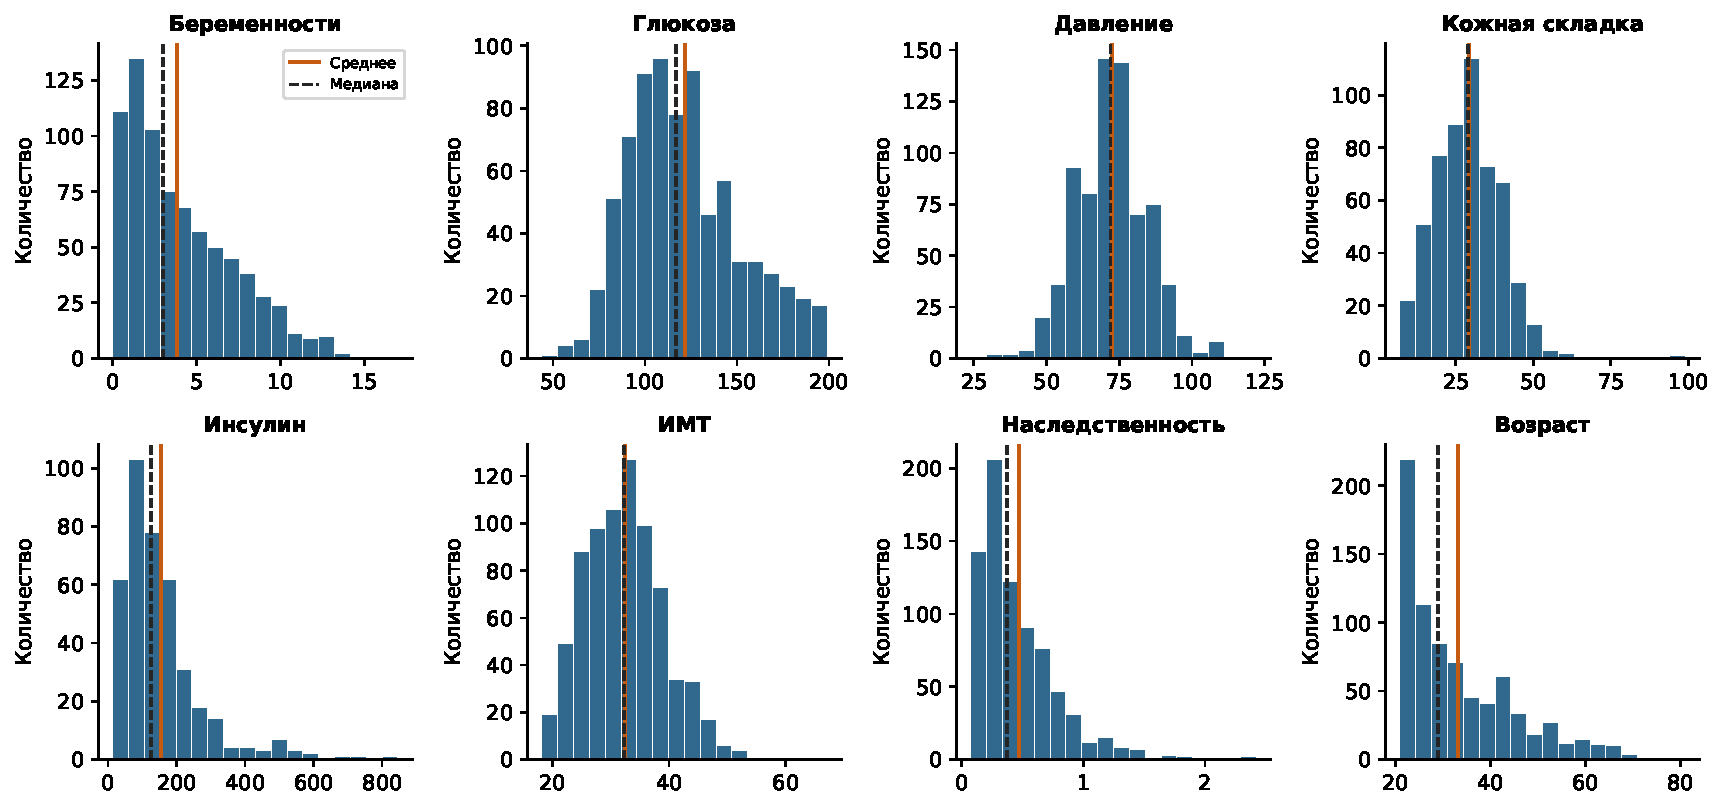
\includegraphics[width=\linewidth]{figures/distributions.pdf}
\caption{Гистограммы наблюдаемых значений; среднее отмечено сплошной линией, медиана --- пунктиром.}
\end{figure}
Инсулин и показатель наследственности имеют выраженные правые хвосты, а шкалы признаков существенно различаются. У Insulin отсутствует $374/768\approx48.7\%$ измерений, у SkinThickness --- $29.6\%$. Медианное заполнение обеспечивает воспроизводимую базовую обработку, но не восстанавливает неизвестные индивидуальные значения и уменьшает вариативность признаков.

\subsection{Разбиение и сетка гиперпараметров}
\begin{table}[H]\centering
\begin{tabular}{lrrr}\toprule Выборка & Всего & Класс 0 & Класс 1\\\midrule
Train & 614 & 400 & 214\\
\quad Fit (часть train) & 491 & 320 & 171\\
\quad Validation (часть train) & 123 & 80 & 43\\
Test & 154 & 100 & 54\\\bottomrule\end{tabular}
\caption{Стратифицированное разбиение; доля test приблизительно 20\%.}
\end{table}
Для GD исследованы $\alpha\in\{0.001,0.01,0.1,1.0\}$ и $T\in\{100,1000,5000\}$: 12 комбинаций. Для Ньютона исследованы $\alpha\in\{0.1,0.5,1.0\}$ и $T\in\{3,10,30\}$: 9 комбинаций. Бюджеты различаются, поскольку одна итерация Ньютона использует гессиан; это не сравнение при равных затратах времени.

\begin{figure}[H]\centering
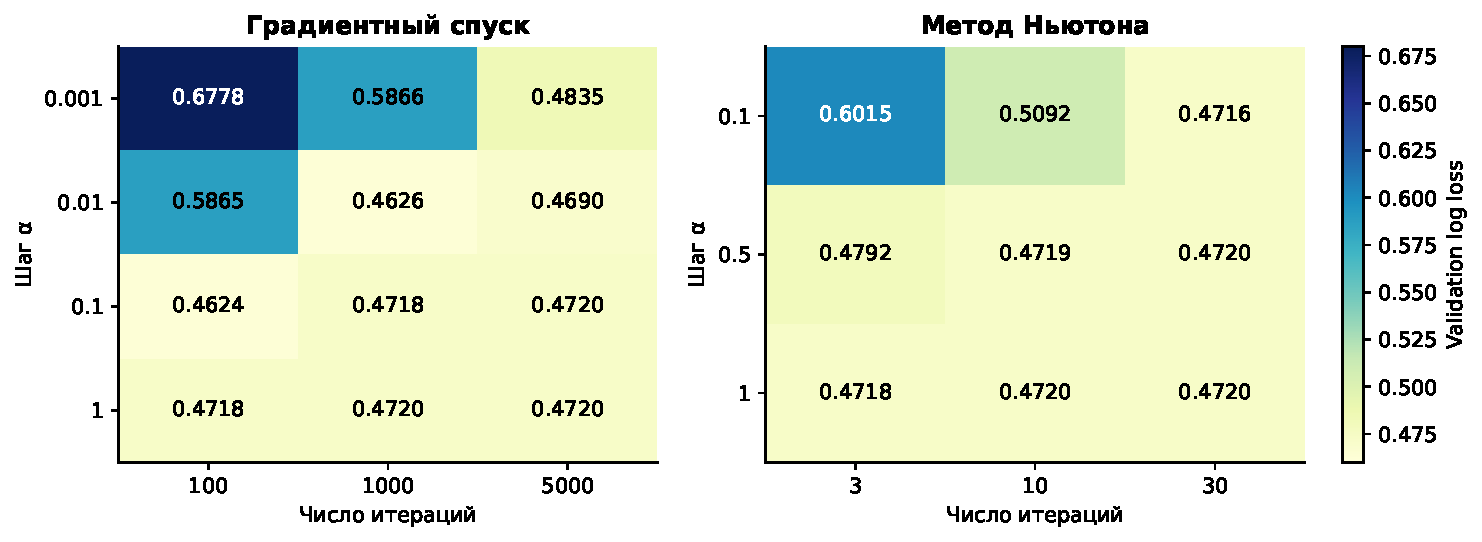
\includegraphics[width=\linewidth]{figures/validation_grid.pdf}
\caption{Log loss на validation для всех 21 комбинации; меньше --- лучше.}
\end{figure}

\subsection{Метрики каждой комбинации}
$L_{val}$ рассчитан после обучения на fit; все остальные показатели ниже --- после независимого переобучения соответствующей конфигурации на полном train. Поэтому это разные обученные модели одной конфигурации. Жирным выделен вариант, выбранный по $L_{val}$, а не по test.

\begin{table}[H]\centering\small
\begin{tabular}{rrrrrrrr}
\toprule
$\alpha$ & T & $L_{val}$ & Accuracy & Precision & Recall & F1 & $L_{test}$ \\
\midrule
0.001 & 100 & 0.6778 & 0.7532 & 0.6600 & 0.6111 & 0.6346 & 0.6788 \\
0.001 & 1000 & 0.5866 & 0.7532 & 0.6667 & 0.5926 & 0.6275 & 0.5965 \\
0.001 & 5000 & 0.4835 & 0.7662 & 0.7045 & 0.5741 & 0.6327 & 0.5103 \\
0.01 & 100 & 0.5865 & 0.7532 & 0.6667 & 0.5926 & 0.6275 & 0.5964 \\
0.01 & 1000 & 0.4626 & 0.7792 & 0.7381 & 0.5741 & 0.6458 & 0.4910 \\
0.01 & 5000 & 0.4690 & 0.7727 & 0.7436 & 0.5370 & 0.6237 & 0.4750 \\
\textbf{0.1} & \textbf{100} & \textbf{0.4624} & \textbf{0.7792} & \textbf{0.7381} & \textbf{0.5741} & \textbf{0.6458} & \textbf{0.4909} \\
0.1 & 1000 & 0.4718 & 0.7727 & 0.7436 & 0.5370 & 0.6237 & 0.4744 \\
0.1 & 5000 & 0.4720 & 0.7727 & 0.7436 & 0.5370 & 0.6237 & 0.4743 \\
1 & 100 & 0.4718 & 0.7727 & 0.7436 & 0.5370 & 0.6237 & 0.4743 \\
1 & 1000 & 0.4720 & 0.7727 & 0.7436 & 0.5370 & 0.6237 & 0.4743 \\
1 & 5000 & 0.4720 & 0.7727 & 0.7436 & 0.5370 & 0.6237 & 0.4743 \\
\bottomrule
\end{tabular}

\caption{Градиентный спуск: все 12 комбинаций.}
\end{table}
\begin{table}[H]\centering\small
\begin{tabular}{rrrrrrrr}
\toprule
$\alpha$ & T & $L_{val}$ & Accuracy & Precision & Recall & F1 & $L_{test}$ \\
\midrule
0.1 & 3 & 0.6015 & 0.7727 & 0.7568 & 0.5185 & 0.6154 & 0.6080 \\
0.1 & 10 & 0.5092 & 0.7597 & 0.7297 & 0.5000 & 0.5934 & 0.5199 \\
0.1 & 30 & 0.4716 & 0.7727 & 0.7436 & 0.5370 & 0.6237 & 0.4764 \\
0.5 & 3 & 0.4792 & 0.7662 & 0.7368 & 0.5185 & 0.6087 & 0.4890 \\
0.5 & 10 & 0.4719 & 0.7727 & 0.7436 & 0.5370 & 0.6237 & 0.4744 \\
0.5 & 30 & 0.4720 & 0.7727 & 0.7436 & 0.5370 & 0.6237 & 0.4743 \\
1 & 3 & 0.4718 & 0.7727 & 0.7436 & 0.5370 & 0.6237 & 0.4744 \\
1 & 10 & 0.4720 & 0.7727 & 0.7436 & 0.5370 & 0.6237 & 0.4743 \\
1 & 30 & 0.4720 & 0.7727 & 0.7436 & 0.5370 & 0.6237 & 0.4743 \\
\bottomrule
\end{tabular}

\caption{Метод Ньютона: все 9 комбинаций.}
\end{table}

Наименьший $L_{val}=0.462361$ получен при GD, $\alpha=0.1$, $T=100$. Конфигурация $\alpha=0.01$, $T=1000$ очень близка: $L_{val}=0.462559$. Разница мала и не подтверждает устойчивого преимущества одной настройки. Порог, признаки и правило выбора не изменялись после просмотра тестовых результатов.

Для выбранной модели Accuracy на test равна $120/154=0.7792$. Базовый классификатор, всегда выдающий 0, имеет Accuracy $100/154=0.6494$ и Recall/F1, равные нулю. Прирост Accuracy составляет 12.99 процентного пункта. При этом выбранная модель пропускает 23 из 54 положительных объектов: сравнительно высокая Accuracy не означает высокую полноту.

\subsection{Влияние гиперпараметров и сходимость}
\begin{figure}[H]\centering
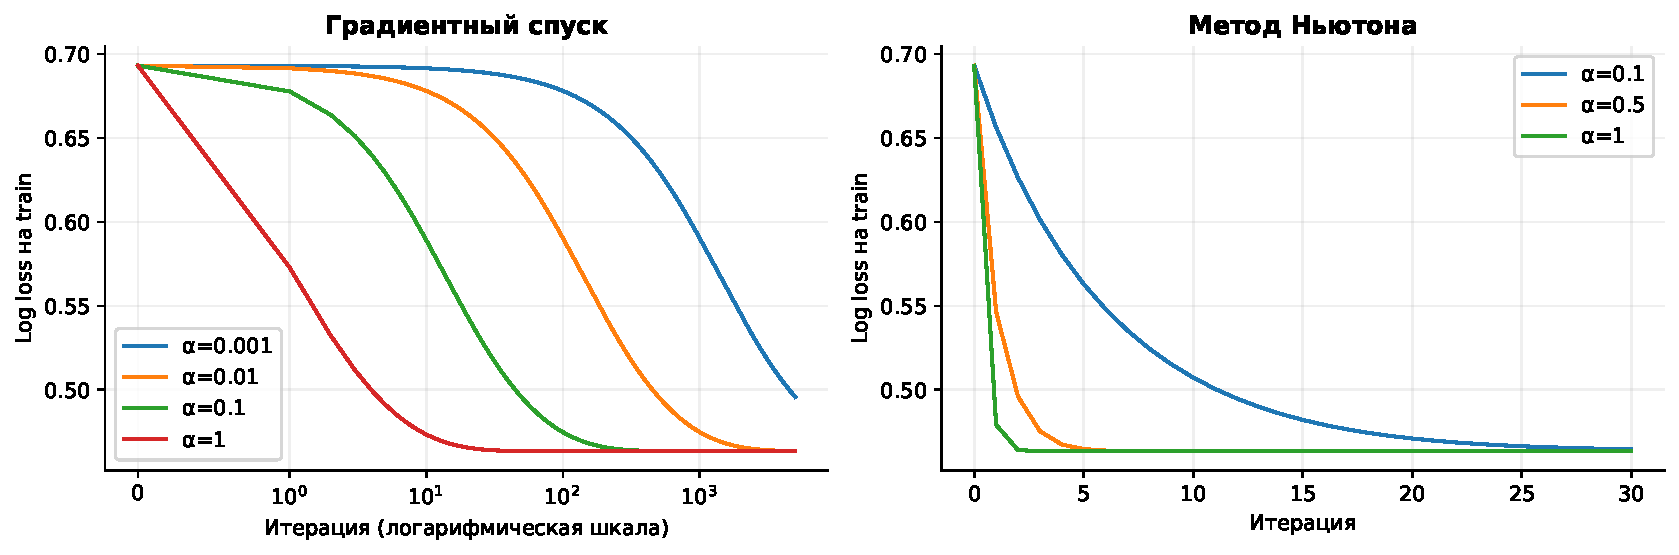
\includegraphics[width=\linewidth]{figures/convergence.pdf}
\caption{Фактическая история train log loss. Для GD показаны запуски по 5000 шагов, для Ньютона --- по 30.}
\end{figure}
\begin{enumerate}
\item \textbf{Шаг GD.} При $\alpha=0.001$, $T=100$ train log loss составляет 0.6781, то есть обучение далеко от минимума. При увеличении бюджета до 5000 он снижается до 0.4958. При $\alpha=1$ уже 100 шагов дают около 0.46347. В проверенной сетке расходимости не обнаружено; это не гарантия для произвольных шагов и данных.
\item \textbf{Число итераций.} Увеличение бюджета уменьшает train log loss, но не обязательно улучшает F1. Например, для GD с $\alpha=0.1$ переход со 100 на 1000 шагов снижает test log loss с 0.4909 до 0.4744, одновременно снижая F1 с 0.6458 до 0.6237. Вероятностная потеря и пороговые метрики оценивают разные свойства.
\item \textbf{Ньютон.} При полном шаге уже три итерации дают train log loss 0.463469, а десять --- 0.463467. Демпфирование $\alpha=0.1$ замедляет сходимость: после трёх шагов потери 0.6014. По числу итераций Ньютон сходится быстрее GD на данном наборе.
\item \textbf{Обобщение.} После достаточного обучения GD и Ньютон дают практически одинаковые потери и одинаковые тестовые классификации. Однако минимум validation достигается раньше полной сходимости. Это согласуется с эффектом ограничения числа итераций как неявной регуляризации, но одного разбиения недостаточно для общего вывода.
\end{enumerate}

\subsection{Выбранная модель и интерпретация}
\begin{figure}[H]\centering
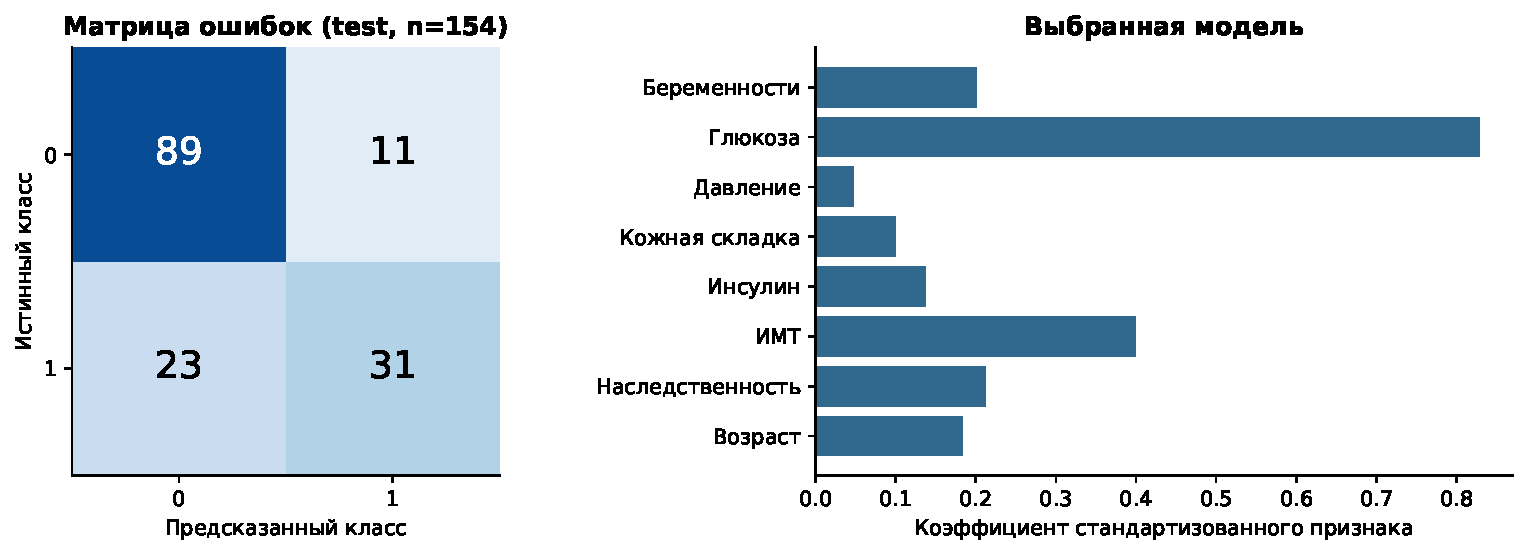
\includegraphics[width=\linewidth]{figures/selected_model.pdf}
\caption{Матрица ошибок и веса модели GD, $\alpha=0.1$, $T=100$.}
\end{figure}
\begin{table}[H]\centering\small
\begin{tabular}{lrr}
\toprule
Признак & $w_j$ & $\exp(w_j)$ \\
\midrule
Intercept & -0.6499 & 0.5221 \\
Pregnancies & 0.2008 & 1.2224 \\
Glucose & 0.8282 & 2.2893 \\
BloodPressure & 0.0469 & 1.0480 \\
SkinThickness & 0.0994 & 1.1045 \\
Insulin & 0.1375 & 1.1474 \\
BMI & 0.3995 & 1.4911 \\
Наследственность & 0.2116 & 1.2356 \\
Age & 0.1829 & 1.2007 \\
\bottomrule
\end{tabular}

\caption{Параметры после стандартизации. Intercept --- свободный член.}
\end{table}
Коэффициент Glucose равен 0.8282: увеличение стандартизованного признака на единицу при фиксированных остальных признаках умножает оценённые шансы на $e^{0.8282}\approx2.2893$. Это отношение шансов, а не множитель вероятности. Положительные коэффициенты описывают условные связи внутри данной модели и не доказывают причинность. Признаки после заполнения масштабируются по train, поэтому единица означает одно стандартное отклонение заполненного обучающего признака.

\subsection{Проверка реализации}
Выполнены шесть автоматических проверок: сигмоида и потери на логитах $\pm1000$; сравнение градиента и гессиана с центральными конечными разностями; ручной пример матрицы ошибок и метрик; отсутствие пересечения частей разбиения и воспроизводимость индексов; неизменность параметров предобработки при обработке новых данных; совпадение решений GD и Ньютона на невырожденном синтетическом примере. Все проверки прошли. Синтетические данные используются только для проверки, а не для приведённых результатов эксперимента.

Предобработка, обучение и метрики реализованы на NumPy и Pandas; Matplotlib применяется для графиков. Готовые алгоритмы классификации, разбиения и расчёта метрик не используются.

\section{Примеры использования метода}
\subsection{Прогнозы на отложенных объектах}
Ниже приведены первые шесть объектов test в порядке исходного индекса CSV. Индексация начинается с нуля; значения не отобраны по правильности прогнозов. Вероятности получены сохранённой моделью с порогом $0.5$.
\begin{table}[H]\centering
\begin{tabular}{rrrr}
\toprule
Индекс строки & Истина & Вероятность & Прогноз \\
\midrule
1 & 0 & 0.0908 & 0 \\
13 & 1 & 0.9033 & 1 \\
15 & 1 & 0.2271 & 0 \\
17 & 1 & 0.2281 & 0 \\
26 & 1 & 0.6473 & 1 \\
39 & 1 & 0.6460 & 1 \\
\bottomrule
\end{tabular}

\caption{Фактические примеры из тестовой выборки.}
\end{table}
Для нового объекта применяются медианы и масштабы, рассчитанные по обучающей части набора. Затем к вектору признаков добавляется единица, вычисляется $p=\sigma(Xw)$ и по порогу $0.5$ назначается класс.

\subsection{Ситуации применения}
Логистическая регрессия полезна как интерпретируемая базовая модель бинарного отклика: вероятность оттока пользователя, отклика на предложение или принадлежности сообщения к спаму. Она удобна, когда нужна компактная модель и объяснение связи признаков с логарифмом шансов. Для таких задач следует заново подобрать данные, предобработку, порог и протокол оценки.

В данном эксперименте решается учебная задача воспроизведения меток исторического набора. Результат не проверен на других популяциях и не предназначен для постановки диагноза. Большая доля пропусков и Recall $0.5741$ ограничивают практическую применимость. Для реального использования нужны внешняя проверка, оценка калибровки и выбор порога по стоимости ошибок на независимой валидации.

\section{Сравнение методов}
\subsection{Сравнительный анализ}
Численно сравнивались два способа оптимизации одной логистической модели. Ньютон быстрее достигает минимума по количеству шагов, GD проще и дешевле на каждом шаге. При достаточной сходимости их качество практически совпадает. Выбор GD с ограниченным бюджетом в этом опыте связан с validation log loss, а не с принципиально большей выразительностью.

Связь с остальными методами модуля можно описать качественно; сопоставимых запусков k-NN и деревьев на данном разбиении не проводилось.
\begin{table}[H]\centering\small
\begin{tabularx}{\linewidth}{lXX}\toprule
Метод & Подходящая задача & Основное ограничение\\\midrule
Линейная регрессия & Количественный отклик и линейные связи. & Не ограничивает прогноз интервалом вероятностей.\\
k-NN & Классификация по близости объектов, локальные нелинейные зависимости. & Чувствительность к масштабу и выбору расстояния; стоимость поиска соседей.\\
Дерево решений & Нелинейные правила и взаимодействия признаков. & Возможное переобучение и нестабильность разбиений.\\
Логистическая регрессия & Бинарный отклик, вероятности и интерпретация шансов. & Линейная граница в пространстве выбранных признаков.\\\bottomrule
\end{tabularx}
\caption{Качественное сравнение назначения методов модуля.}
\end{table}

\subsection{Примеры лучшего использования}
Для прогноза непрерывной стоимости естественна линейная регрессия; для локально похожих объектов при разумной метрике можно рассматривать k-NN; для правил с порогами и взаимодействиями --- дерево. При бинарном отклике и необходимости объяснять вклад признаков логистическая регрессия даёт удобную отправную точку. Эти рекомендации описывают свойства методов, а не установленное экспериментом превосходство на всех данных.

\section{Заключение}
Поставленная задача выполнена: загружен реальный датасет, исследована статистика, обработаны отсутствующие измерения, реализована логистическая регрессия с нуля и оценена 21 комбинация гиперпараметров. Градиент, гессиан и метрики проверены независимо от основного эксперимента.

По заранее выбранному критерию validation log loss отобрана конфигурация GD с $\alpha=0.1$, $T=100$. После обучения на 614 объектах она дала Accuracy 77.92\%, Precision 73.81\%, Recall 57.41\% и F1 64.58\% на 154 тестовых объектах. На практике существенны не только правильные классификации, но и 23 пропущенных положительных объекта.

Метод Ньютона оказался эффективнее по числу итераций до близкого к минимуму train log loss. Увеличение числа шагов не обеспечивало улучшения всех метрик. Результаты относятся к фиксированному разбиению: для более надёжного выбора параметров целесообразны повторная стратифицированная кросс-валидация, исследование регуляризации и независимая проверка качества вероятностей. Настройки нельзя объявлять универсально лучшими на основании этого опыта.
